\documentclass{article}
\usepackage[draft]{SRM2}
\usepackage{graphicx}
\usepackage{url}

\title{The AviaNZ Birdsong Analysis Software (v 1.3)}
\author{The AviaNZ Team \\(\url{stephen.marsland@vuw.ac.nz})}
\date{October 2018}

%\usepackage[usenames, dvipsnames]{color}

%Revise with track changes
\usepackage[markup=default]{changes}
%\usepackage[final]{changes}
\usepackage{soulutf8}

\begin{document}
\maketitle

%Shift-click, ctrl-click
%scroll bar, menus not buttons

%Operater and reviewer
% 5 areas bit
% not a problem

This is a brief guide to version 1.3 of the AviaNZ program. 
We really want feedback on it, particularly what works and what doesn't, how you would like to see it improved, and what other functionality it needs. We are more than happy to talk about our plans as well. 

%If you haven't done any birdsong processing before, make sure that you read Section~\ref{labelling}, which works through an example. 

\section{Getting Started}

{\em In contrast to previous versions, this version of AviaNZ does not require you to run it as administrator in Windows. It places some files in the home directory of your computer; in \url{C:/Users/username/AppData/Roaming/AviaNZ} for Windows and \url{~/.avianz} for Mac and Linux.}

When the program loads, you are presented with three options in the following start-up screen:

\begin{figure}[h!]
\centering
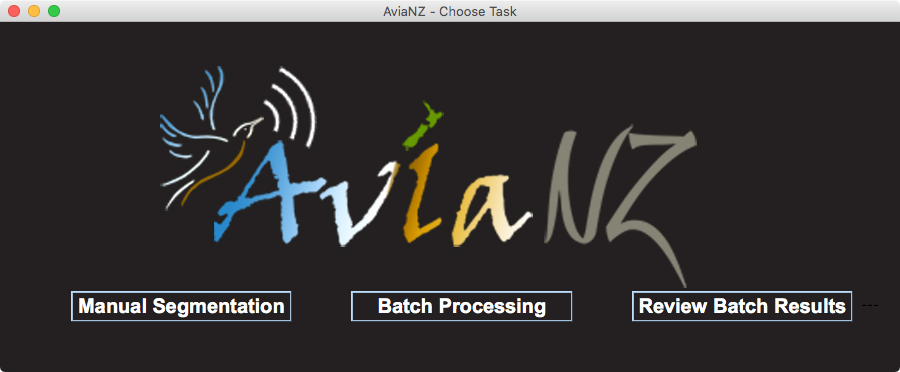
\includegraphics[width=.3\textwidth]{Figs/splashscreen}
%\caption{\added{Starting window of the program.}}
\label{welcome}
\end{figure}

The first option (Manual Segmentation) is described more in Section~\ref{sec:manual}. It enables you to see and manually process audio files. The second option (Batch Processing) takes whole directories (and subdirectories) of audio files and automatically segments the bird calls of a particular species; see Section~\ref{sec:auto}. You can view the output of this automatic segmentation using the first option; the software also produces an Excel file showing the results, see Section~\ref{sec:outputs}, but in addition the third option (Review Batch Results) enables you to check the results of the batch processing easily. 

\section{Manual Segmentation}
\label{sec:manual}

If you select manual segmentation, you will see a dialog box asking you to select a file to view. Use this in the normal way to select a sound file from a directory. Once you have selected one, the program will ask you to give names for the operator and reviewer. These are useful to keep track of who has looked at different files. Following that, you should see a screen like the one below (Figure~\ref{main}). This is the main program for manually labelling birdcalls, or reviewing the processing of automatic processes.

The program automatically loads the first 5 minutes of a file. 

\begin{figure}[h!]
\centering
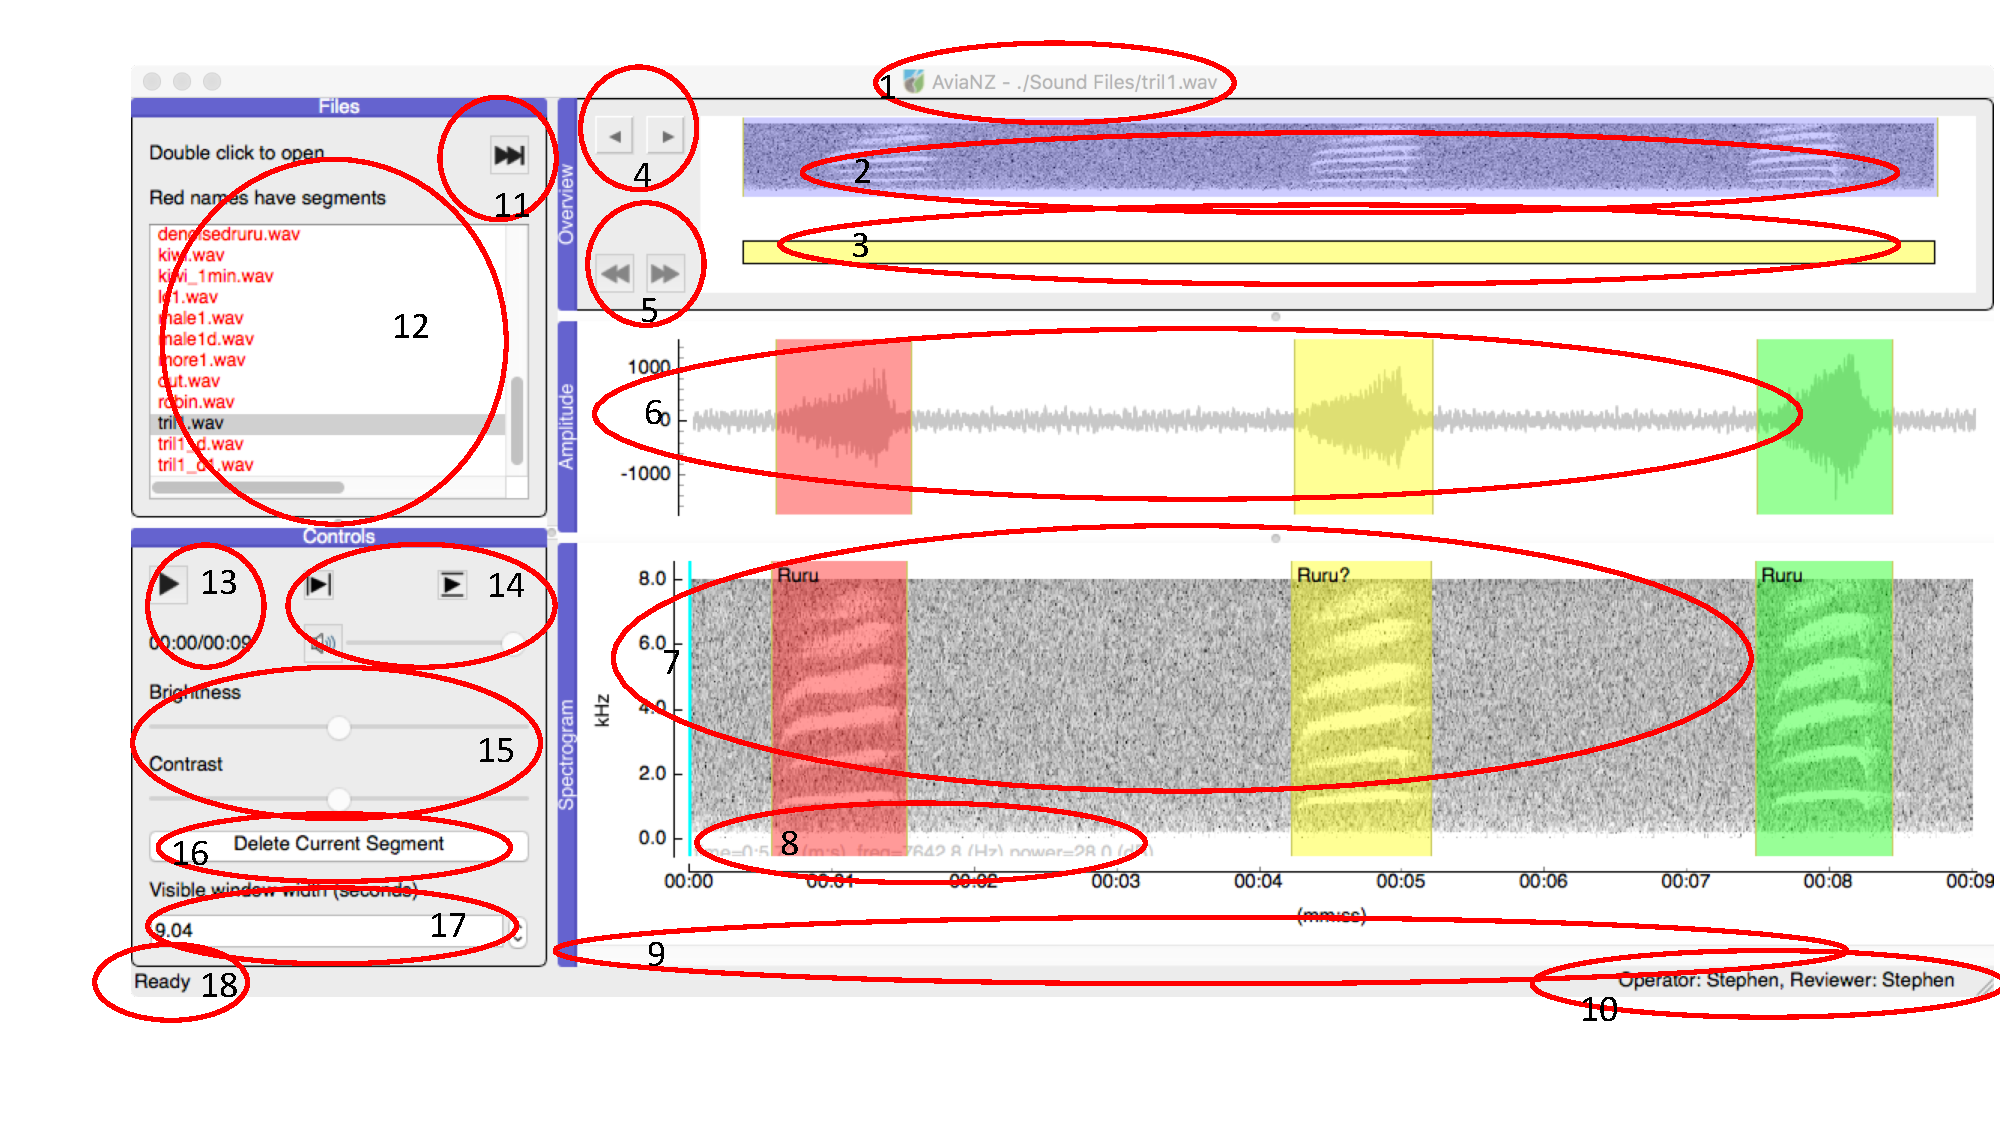
\includegraphics[width=.8\textwidth]{Figs/AviaNZInterface.pdf}
\caption{The interface for manual birdsong annotation and analysis.}
\label{main}
\end{figure}

\newpage
\begin{itemize}
\item There are five separate areas of the screen within the AviaNZ program (each of which has its name in a blue bar). They are:
	\begin{description}
	\item[Overview] This shows you a picture of the 5 minutes of the file (labelled 2 in the figure). The part you are looking at in the main plots is shown in blue (it's actually the whole file in the example figure). Below it there is a coloured bar (labelled 3 in the figure, and in yellow). There are left and right arrow buttons (labelled 4) and double arrow buttons (labelled 5) on the left of this area. The single arrow buttons move the view in the main area along, while the double arrow buttons move to the previous 5 minutes or to the next 5 minutes of the file (if it exists). 
	\item [Files (12)] This is a list of files in your current directory. You can double-click on one to select it and open it. Files in red have been annotated, files in black have not. The double arrow button on the top right of this area (labelled 11) moves on to the next file.
	\item[Amplitude plot (6)] This shows a picture of the sound file. It's one of the two parts of the interface that you can use to label the birdcalls. If you don't want to see it, you can hide it using the Appearance menu by selecting `Show amplitude plot' so that it is not ticked.
	\item[Spectrogram plot (7)] This is the second picture of the sound file, and the one that has more information and is most useful. It is possible to display information about where the mouse is pointing on the spectrogram (time, frequency, energy value; 8 in the figure) by choosing `Show pointer details in spectrogram' from the Appearance menu, and to switch it off the same way. There is also a scroll bar to move through the file (9). 
	\item[Controls] These play the sound file, and modify the appearance of the plots (13--17 in the figure), see Section~ref{sec:controls}.
	\end{description}

In addition, there are two extra parts to the interface:
	\begin{description}
	\item[Menu] The menu at the top of the screen. The name of the current file is shown in the title of the window (1).
	\item[Bar at the bottom] At the very bottom of the screen there is an area (marked 18) that gives any status updates from the program, and on the right, information about the currently selected Reviewer and Operator (marked 10).
	\end{description}

\item You can drag the five screen areas around and reorder them if you wish, by dragging the blue bar on the top or left of them. You can also make them into their own windows by double-clicking on the blue bar. If you decide that you made a mistake doing that, then there is an option in the Actions menu to `Put docks back' that returns them to the original configuration.

\item To load a new file, either choose `Open sound file' in the File menu, or just double click one in the Files screen area (double clicking on a folder will open that folder), or click on the button labelled 11 to move to the next file. 

\item If you want to move to a new directory, either use the `..' option at the top of the list of files to navigate around your computer's file system, or use the  `Open sound file' in the File menu.

\item To restart the program, for example so that you can start doing some batch processing, choose `Restart' from the File menu. To quit completely, choose `Quit'. 

%\item The program will tell you if it is doing anything by putting text in the area labelled 18. \added{The selected operator is shown at the bottom of the window (10).}

\subsection{Spectrogram and Amplitude}

\item The two main plots (Amplitude and Spectrogram; 6 and 7) show a section of a sound file. The part you are looking at is highlighted in blue in the top (Overview: 2) picture. Sometimes people only want to look at the spectrogram. If you are one of these people, in the Appearance menu there is an option `Show amplitude plot', which is initially ticked. Click on it to remove the tick and the amplitude plot will vanish. If you change your mind, choose the option again. You can also hide the list of files (12) and the annotation overview (3) in the same way. AviaNZ will remember your choice in future uses.

\item Sometimes spectrograms don't look good initially, for example because of high noise. You can modify the brightness and contrast of the spectrogram using the two sliders marked 15 in the figure. You can also use a different colour scheme, and invert the colour map (swap black and white), by choosing the relevant options in the Appearance menu. 

\subsection{Zooming and Scrolling}

\item The part of the file you can see can be changed by:
	\begin{itemize}
	\item dragging the scroll bar below the spectrogram (9)
	\item clicking on the left or right arrows on the right of the Overview picture (labelled 4)
	\item dragging the blue highlight in the Overview picture itself (labelled 2). 
	\item clicking on any of the boxes in the bar below the Overview picture (labelled 3)
	\item pressing the left or right arrow keys
	\end{itemize}
	The amount of the file that you can see (the visible width) can be changed by either: 
	\begin{itemize}
	\item dragging the ends of that blue highlight in (2)
	\item changing the `Visible window width (seconds)' in the Controls dock (labelled 17) by clicking on the up and down arrows, or typing in a new number.
	\end{itemize}

\item You can also view a restricted amount of the spectrogram by reducing the visible frequency band. To do this non-destructively, use the `Change spectrogram parameters' dialog in the Appearance menu, and change the Lowest and Highest Frequency options.

\subsection{Moving Through Long Files}

\item If files are longer than 5 minutes, use the double arrows labelled (5) to move to the next or previous sections, or press shift + left or right arrow keys. Note that there is a 10 second overlap between the files. You can change the page size and the amount of page overlap by choosing the relevant options in the `Interface Settings' in the Interface menu, as will be described later. The times on the axis below the spectrogram show locations in the full file. Note that operations like denoising and segmentation apply to the visible 5 minute portion of the file, not the whole file. 

\subsection{Playing the Sounds \label{sec:play}}

\item You can play the sounds visible on the screen using the `Play' button at the top-left of the Controls section (labelled 13). The button turns into a `Pause' button while playing (or you can press the `Escape' key). The light blue bar in the spectrogram plot (7)  shows where the playback is up to. When paused, you can drag this bar if you want to hear a particular part of the file. Move the mouse over it, and the bar will go red. Then click and drag to move it. The time below the play button shows the length of the file and the current position of the blue bar in minutes and seconds. You can change the volume of playback using the slider in (14). 
You can also play a segment of sound, assuming that a segment is selected. We will cover this below.

\item To stop playback and have the slider return to the start of the visible section, press the Stop button instead.

\item When a segment is selected (so that it is blue -- segments are covered next) you can use the two play buttons in 14 in the picture to play just that small segment. The difference is that the one on the left plays all the frequencies in the sound file, while the one on the right will play only the frequencies highlighted, so that you can isolate particular frequencies of a call. This is particularly helpful when there is high level of background noise that is in a particular frequency range, such as cicadas, or where there are overlapping calls in different frequency bands.

\subsection{Performing Segmentation}

\item Segmentation has changed slightly in this version of the software. 

\item You select and edit a segment by clicking on it with one of the mouse buttons (left or right), and create one by using the other mouse button. You can select which performs which action using the `Mouse settings' of the `Interface settings' in the Appearance menu.

\item There are three options for how to create a segment. You select one of them in the `Mouse settings' of the `Interface settings' in the Appearance menu:
	\begin{itemize}
	\item Start and stop a full frequency band by clicking (i.e., click once at the correct time for the start of a segment, move the mouse to the end, click again, the box covers all frequencies)
	\item Start and stop a limited frequency band by clicking (i.e., click once at the correct time and frequency (in the spectrogram) for the start of a segment, and then again at the time and frequency for the end)
	\item Drag a limited frequency band box (i.e., click and hold the mouse button and drag the mouse to the correct end point in both time and frequency)
	\end{itemize}

\item While the segment is being made, it is red. At the end it will turn blue, and a drop-down menu will then appear asking you to label the segment. 

\item To choose the type of bird, click on the name. If the type isn't in the list, move to `Other'. If it isn't in the second list, at the bottom of that list is a selectable box (it probably says `Albatross'). Clicking on it provides the complete list of birds. If there is something missing from there, choose 'Other' from it, which is at the very end. It will ask you to enter a name. From then on this name will appear in the list. If you click anywhere on the screen except on a bird name in the menu then the menu will disappear and the bird type will be labelled as `Don't Know'. 

\item By default these lists update dynamically, so that bird types you have chosen appear at the top of the list. If you don't like that, then you can disable it in the `Interface settings'. 

\item If you find that the colours make it hard to see the data underneath the boxes you can make them transparent using the `Make dragged boxes transparent' option under `Annotation' in the `Interface settings'. You can also choose different colours if you have particular preferences.

\item If you select a segment that already exists then it will turn blue and the menu will reappear so that you can correct mistakes.

\item You can avoid seeing the menu by pressing the shift key on the keyboard when you click to finish the segment. The program will then give the segment the same label as the previous box that you labelled. This is very useful when there is one bird calling repeatedly.

\item You can also show that you are uncertain by pressing the control button when you click to segment (command button on a Mac computer). The names of the birds will then have a question mark after them. 

\item By default, the software only allows one bird type to be specified for each segment. However, there may be times when you wish to label multiple species in one box (for example, for the dawn chorus). In that case, choose `Default to multiple species' in the `Interface settings'. Now, when you choose a bird from the list it will be ticked, and the menu will not close automatically, allowing you to make multiple selections. To unselect something, click on it again. When you make a new segment, `Don't Know' if selected by default. Choosing any other option deselects `Don't Know'. You can reselect it if you do want that it in the list. 

\item The segments that are drawn on the screen have different colours. They are changeable in the `Interface settings', but by default are:
	\begin{description} 
	\item[Blue] This segment is currently selected. You can play it by pressing the buttons in 14, or give it a new label. 
	\item[Green] This segment has been labelled with a bird name.
	\item[Yellow] This segment has been labelled with a bird name with a question mark.
	\item[Red] This segment has been labelled as `Don't Know'.
	\end{description}

\item These colours match the rectangles underneath the overview (labelled 3). For each 10 second segment of the file, these boxes are:

	\begin{description} 
 	\item[White] if there are no segments, 
	\item[Red] if there are `Don't know' segments, 
	\item[Yellow] if there are question marked segments, or 
	\item[Green] if all the segments in that section are labelled with definite species. 
	\end{description}
	
\item You can click on those rectangles in (3), and they will update the amplitude and spectrogram plots to show that section of the file. This is a good way to move through the file quickly.

\item Segments can be moved by dragging them, or resized by dragging the left and right ends, just like the Overview highlight. For bounded-frequency boxes, drag the handle on the top right corner of the box to resize. (All these interactions use the non-drawing mouse button.)

\item Segments can be deleted by selecting them (so that they turn blue) and then clicking on the `Delete Current Segment' in the Controls (16). You can also just press the delete or backspace key on the keyboard. 

\item To delete all of the segments, use the `Delete all segments' option in the Actions menu. 

\item Segments are saved automatically, so that you can't lose your work.

\end{itemize}

\subsection{Menu Options}	

\subsubsection{{\em Appearance Menu}}

\begin{description}
\item [Changing appearance] The first four options in the menu hide or reveal the amplitude plot (6), list of files (12), annotation overview (3), and information about where the mouse is pointing in the spectrogram (8). 
%\item [Drag boxes] This option enables the user to select if they wish to perform segmentation by clicking on the start and end of a segment, or dragging a box. The boxes can be made transparent, when only their edge shows the colour code of what kind of label they have been given.
%\item[Invert Spectrogram] This is currently a play feature that shows that it is possibly to invert a spectrogram to get a new wave file. The spectrogram picture will update to be a bit blurred. 
\item [Choose colour map] This enables the user to select a colour map they prefer to the standard grey one. There is also an option to swap black and white (inverting the colour map). 
%\item [Make frequency axis tight] After bandpass filtering, this updates the spectrogram plot to stop showing the empty bands.
\item [Change spectrogram parameters] A set of options to modify the spectrogram. Enables changes of the windowing function, width and increment of the FFT, and the option to not subtract off the mean. The `Multitapering' option can make very noisy spectrograms look better, but it takes a lot of computer time. The two sliders at the bottom of the dialog enable the user to non-destructively show a limited frequency band in the spectrogram. The axis in the plot shows what is visible. 
\item [Make read only] When reviewing a segmentation it is possible to click on the plots by mistake, adding further segments. This option avoids this problem. It can be turned off by selecting it again. 
\item [Interface settings] This option enables the user to customise several things about AviaNZ, such as the annotation colour scheme, length of the annotation overview sections, and auto save frequency. The user can also choose how much of a file is loaded automatically. There is a tick box under `Human classify` labelled `Save corrections'. This option is used when reviewing the automated segmentation results  (see Section \ref{sec:action} and Sections \ref{sec:auto}--\ref{sec:outputs}). It is also possible to change the lists of birds you are using. 
There is an option to set the operator and reviewer, this facility can also be found in the File menu.
\end{description}

\subsubsection{{\em Actions Menu}}
\label{sec:action}

These options will mostly provide dialog boxes that ask you to make choices. 

\begin{description}
\item [Delete all segments] Does what it says. 
\item [Denoise] Runs some programs that try to get rid of the noise in the sound file so that the birdcalls are easier to see. 
\item [Add metadata about noise] Allows the user to specify if the sound file is particularly corrupted by noise, and also to identify the type(s) if known. This can be an optional datafield, or made compulsory for each file by choosing the appropriate option in the `Interface settings'.
\item [Show fundamental frequency] Plots an estimate of the fundamental frequency for each call as a red line on the spectrogram.
\item [Segment] You can ask the computer to segment the calls automatically. 
We currently provide 3 options, and you can try them to see how well they work.
%\item [Find Matches] If you select a segment (so that its box is green) and then press this button the program will look for others that are similar. It does not currently deal well with nosie. 
%\item [Filter Spectrogram] This tries to clean the spectrogram for easier viewing.
\item [Human Review] These two options provide two different ways to view the segments and their labels for easier checking. The option to Show all pages (in `Interface settings') decides on whether to view segments in an entire file, or just the current 5 minutes of it. 
	\begin{description}
	\item [Human Review [All segments]] This option shows the segments one-by-one in time order (Figure~\ref{check1}).
	\begin{figure}
	\centering
	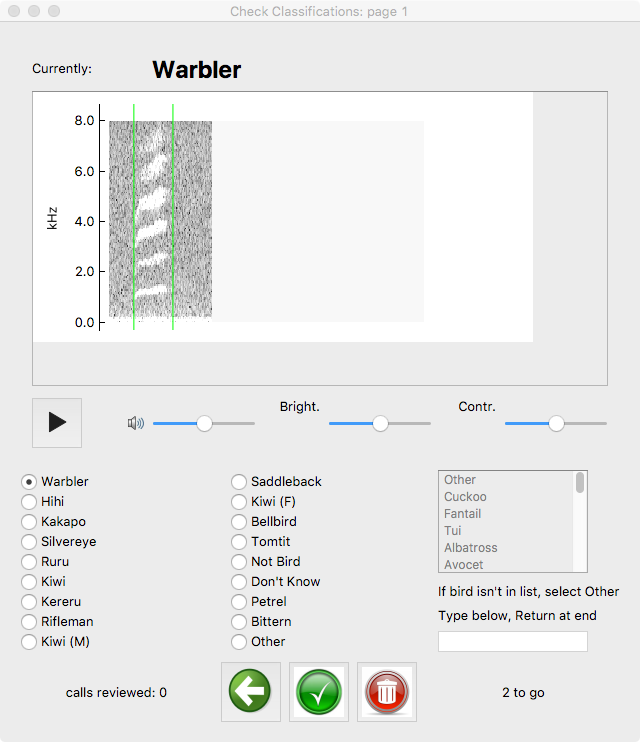
\includegraphics[width=.6\textwidth]{Figs/review1}
	\caption{Example of outputs for Human Review [All segments].}
	\label{check1}
	\end{figure}
	To play the segment, click on the play button. Green bars mark the limits of current segment, and a couple of seconds of context are provided around it. You can also change the spectrogram brightness to make it easier to review. If the label is correct, click on the green tick, which will make the next image load. If not, select the correct label before clicking the tick button. If you have allowed multiple species selection you can pick several options. To delete a segment, click on the red dustbin button. To move back to the previous one, click the back arrow; note that this will not save your current changes. 
	\item [Human Review [Choose species]] This option asks you to choose a bird from those found in the current file. For each segment that is wrongly labelled, click on its picture (the colour map will change). These segments will be deleted (Figure~\ref{check2}). By default, the program will automatically save the corrections in a temporary folder so that they can be used to help us improve these classifications in the future. You can stop this behaviour in the `Interface settings' interface. You can change the brightness and contrast here as well, and also play the sounds by hovering on the image, and then clicking on the play button when it appears. 
	\begin{figure}
	\centering
	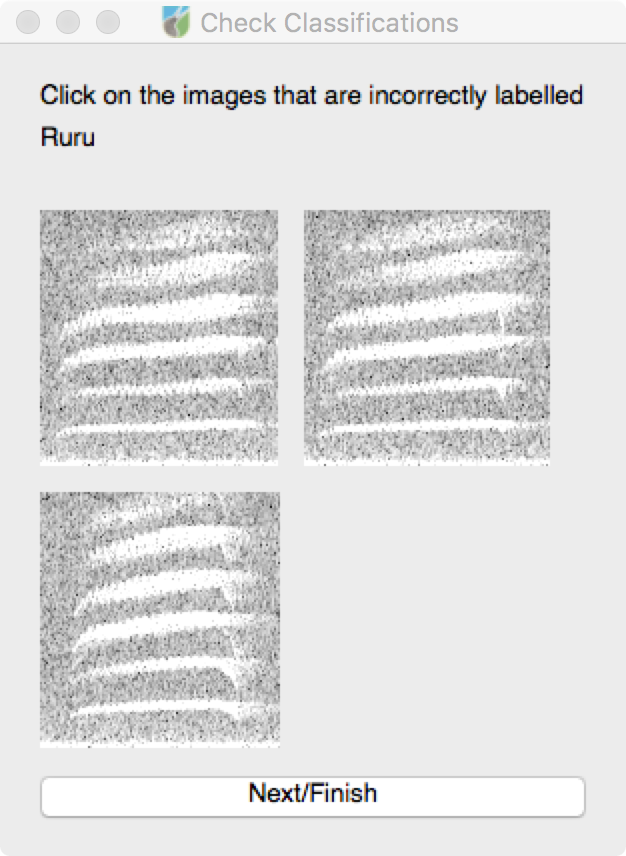
\includegraphics[width=.4\textwidth]{Figs/Check2}
	\caption{Example of the window for Human Review [Choose species].}
	\label{check2}
	\end{figure}
	\end{description}

\item [Export segments to Excel] This enables the user to save a summary of the annotation of the currently opened file into an Excel workbook (in the same location as the current sound file), as is described in Section~\ref{sec:outputs}. 
\item [Save as image] Saves the spectrogram currently visible on the screen as an image.
\item [Save selected sound] Saves a selected segment as a short sound file.
\end{description}

\subsubsection{{\em Help Menu}}

\begin{description}
\item [Help] Gives access to this file.
\item [Cheat sheet] Provides a set of examples of common bird calls. 
\end{description}


\section{Automatic Segmentation of a Folder}
\label{sec:auto}

\begin{itemize}
\item If you select `Batch Processing' from the starting window, you will see a screen like the one below (Figure~\ref{batch}). Navigate to a folder containing recordings to process. If this folder contains subfolders, the program will work through all of the folders inside the original one. It ignores any files that already have annotations. Choose the species that you are interested in detecting from the drop down list, or select `All Species'. 

\item Press the `Process Folder' button to start the program. Note that this is a very computationally intensive process, and will take a long time (hours) if there are lots of files to process, and make your computer hard to use for anything else. 

\item If you stop the processing partway through, AviaNZ will try and restart from the place it got up to last time if you restart it.

\item Once it has finished, the window will close and the AviaNZ start screen will reopen so that you can review the outputs. You can either do this in the manual review interface, or use the `Review Batch Results' option in the starting screen. A similar menu to the `Batch Processing' option will prompt you to select a folder with previously processed files. If you choose `All species' then you will see a screen like Figure~\ref{check1}, while if you select a particular species, you will see a screen like Figure~\ref{check2}. 

\item AviaNZ also produces an Excel spreadsheet, as is described in Section~\ref{sec:outputs}. Note that the `All species' option will delete the Excel files for individual species to ensure that everything is consistent. The information is then held in the one spreadsheet.  
\end{itemize}
	
\begin{figure}[h!]
\centering
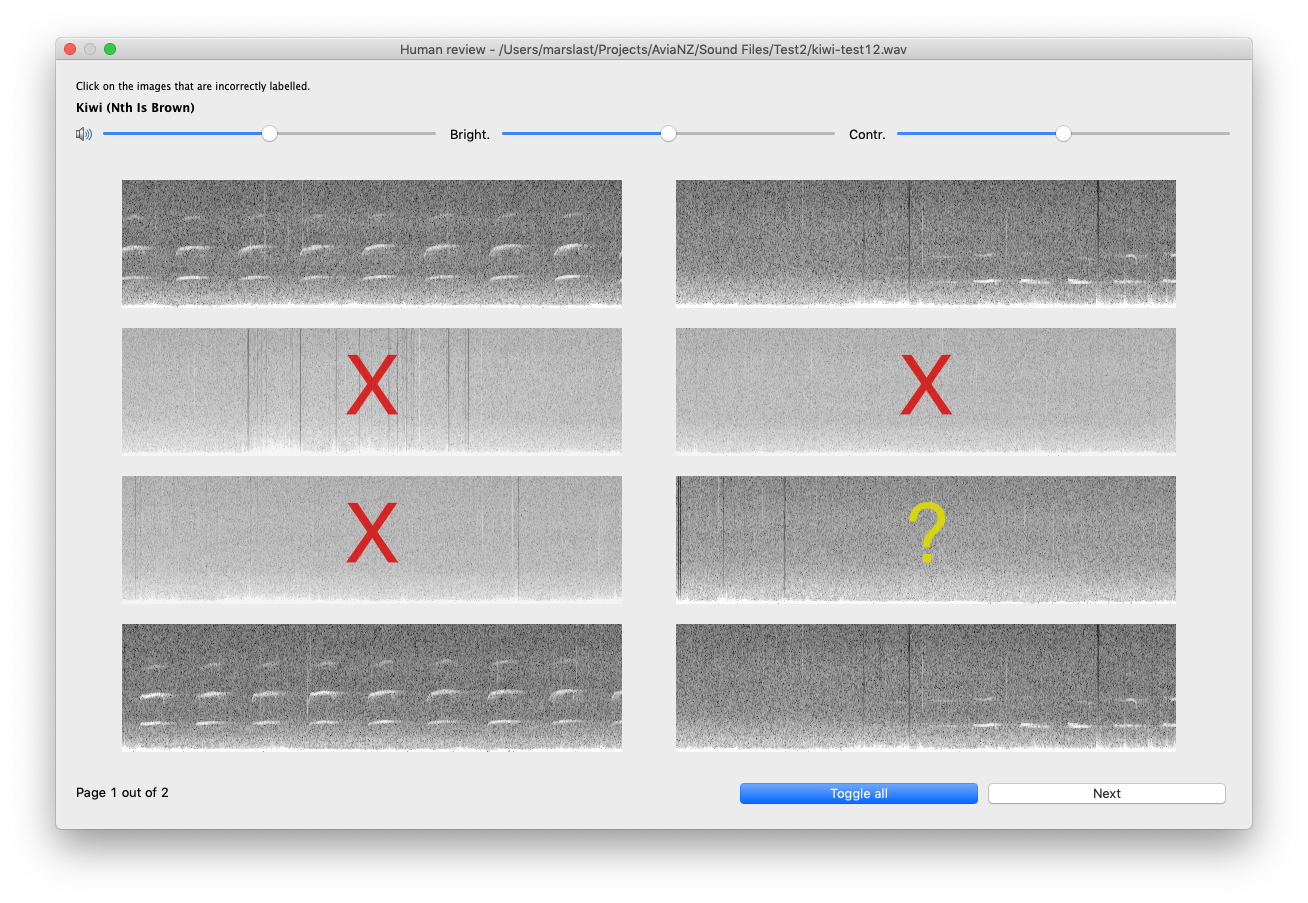
\includegraphics[width=.5\textwidth]{Figs/review2}
\caption{The interface for batch processing.}
\label{batch}
\end{figure}

%\begin{figure}[h!]
%\centering
%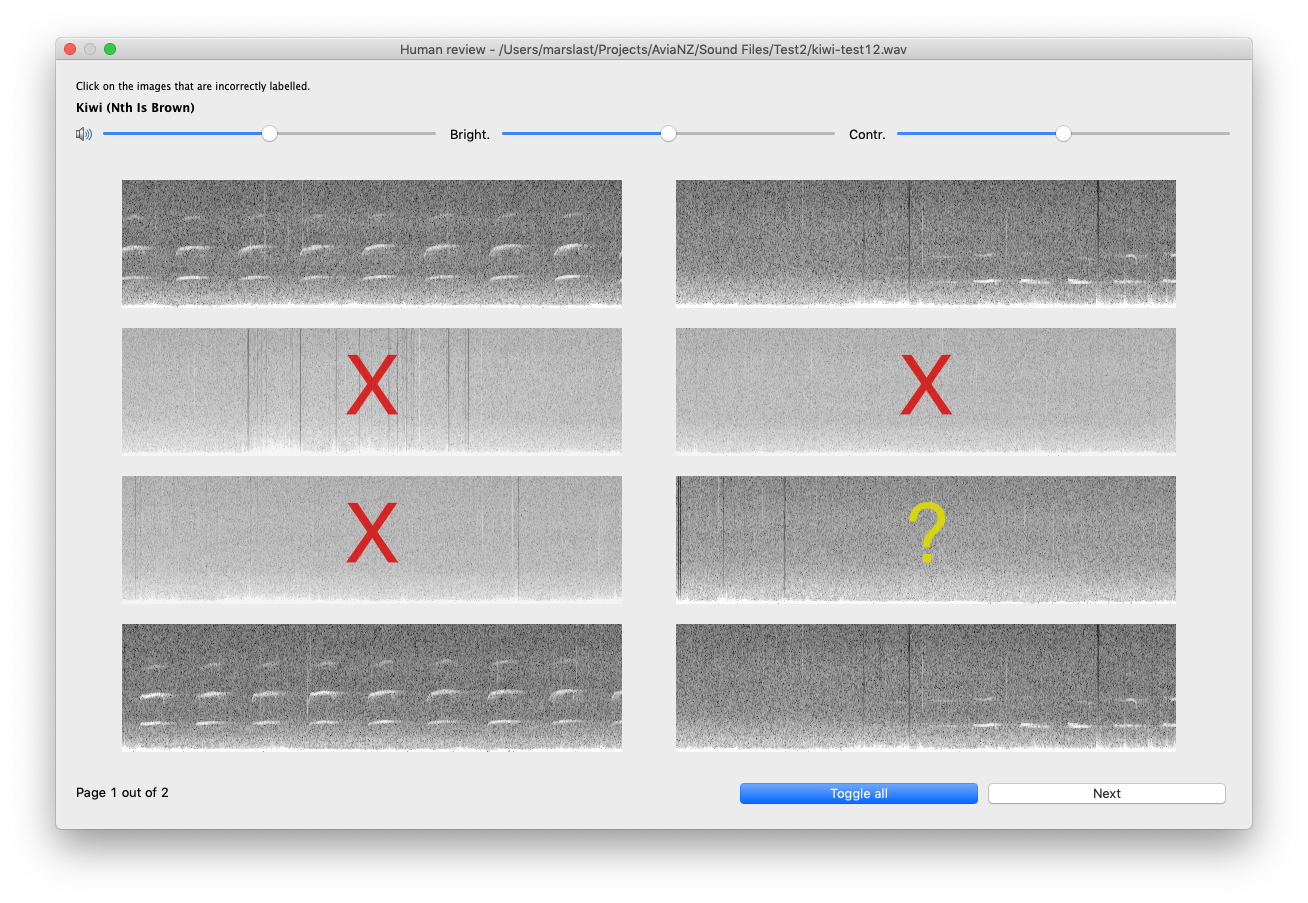
\includegraphics[width=.5\textwidth]{Figs/review2}
%\caption{The interface for batch processing.}
%\label{batch2}
%\end{figure}

\section{Outputs}
\label{sec:outputs}

\begin{itemize}
\item The AviaNZ program aims to provide detailed and easy-to-review outputs. An Excel file (with the name `DetectionSummary' followed by species selected) will be generated with three sheets of outputs in the same directory as the files. If this file already exists, the new results will be appended to the end of each sheet. 

\item The three sheets of the Excel workbook are:

\begin{enumerate}
\item start and end times of each birdcall detected
\item presence/absence of the target species (or set of species) in each recording
\item  presence/absence of the target species (or set of species) in each time interval that the user specifies (by default 60 seconds)
\end{enumerate}

\item In addition to the Excel file, for each sound file AviaNZ generates an annotation file of the automated detections that  the user can open and review in either the main interface or using the `Review Batch Results' option. 
\end{itemize}

%\section{A Walkthrough}\label{labelling}
%
%This section shows you how I use the software to perform labelling. 
%
%\begin{itemize}
%\item When the program starts, choose `ruru.wav' from the list of files. This is a five minute file, and quite noisy, and it has lots of calls in it. 
%\item The two main plots show you the first 10 seconds of the recording. In the spectrogram plot, the grey speckle is noise, and the white marks inside it are the calls. Mostly people recognise the type of bird by identifying the patterns in these pictures. You should be able to see five calls, and then some noisy silence. I've highlighted the calls in this picture:
%
%\begin{figure}[h!]
%\centering
%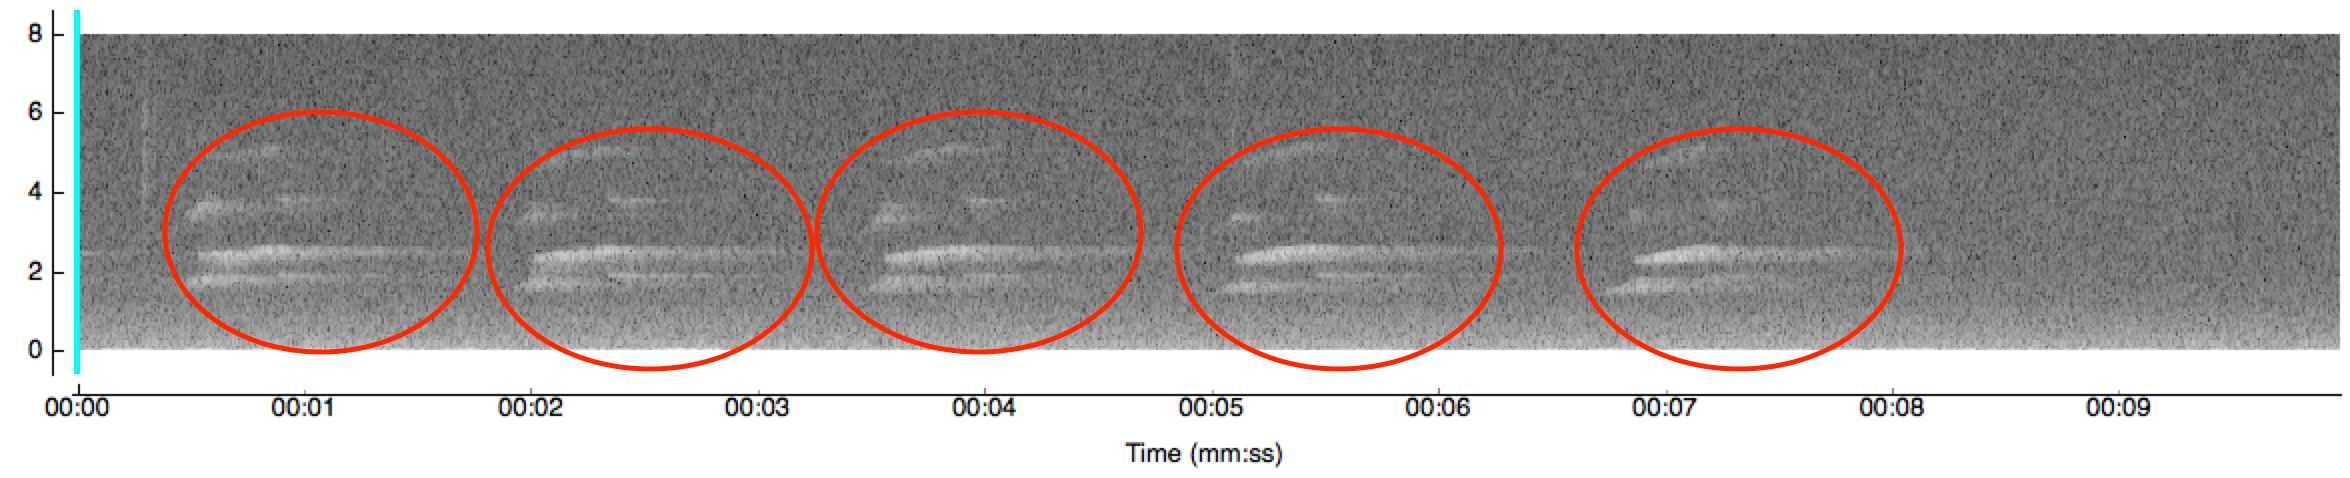
\includegraphics[width=.8\textwidth]{ruru}
%\end{figure}
%
%\item If you want to hear the calls, click on the play button (and make sure that the volume is turned up on your computer). 
%\item Play with the `Brightness' and `Contrast' sliders (12) in Figure 1 until you find it easy to see the birdcalls. If you want to make the calls be in black instead of white, click on the  `Invert colour map' option in the Appearance menu. You can also change to a different colour scheme there. I chose the options to make it look like this:
%
%\begin{figure}[h!]
%\centering
%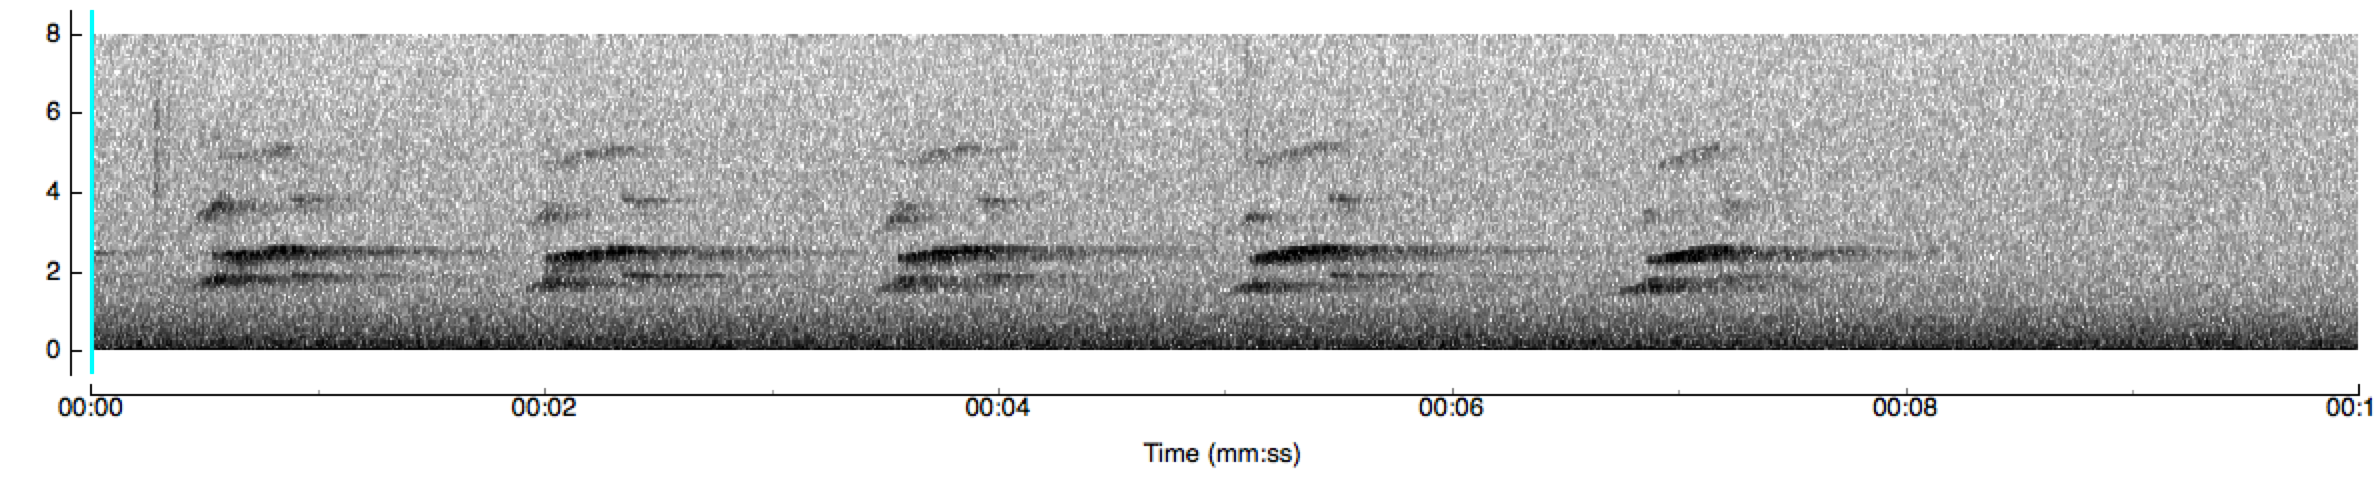
\includegraphics[width=.8\textwidth]{ruru2}
%\end{figure}
%
%\item Decide if you like seeing 10 seconds. If you prefer a different length, either: (1) drag the end of the box in the overview picture (at the top of the screen) in or out, or (2) make the length of time in `Visible window length' longer or shorter. The plots will update automatically. 
%\item Now we are ready to start to segment and label the calls. Click once with the mouse near the start of the call. Then move the mouse so that the blue box appears, and click again near the end of the call. In the drop-down box of bird names, click on `Ruru'. 
%\item If you decide you missed the start or the end, you can drag the ends of the box by putting the mouse over them, then clicking and dragging them. You can also move the whole box. 
%\item Move on to the next call and repeat.
%\item If you think that this second call is also a ruru, press shift when you click the second time, and the menu won't drop down, and the box will also be labelled as 'Ruru'
%\item If you aren't sure about a call, but think it is probably a ruru (or whatever bird) press control when you click and the menu options will have question marks on them. 
%\item When you have labelled all of the calls, press the arrow button at the top-right of the screen to move on to the next part of the recording, or drag the slider at the bottom of the screen, and carry on. 
%\item When you have finished a file, click on `Load File' to load another file, or click on `Quit' to close the program. 
%\end{itemize}
%
%When doing this you will realise what a slow and laborious procedure it is. That's why we want to automate most of it. Unfortunately, the amount of noise in the files makes it hard. You can try the different algorithms under `Segment' and see if any of them work well for your files, but for this example, which is quite noisy, they make a lot of mistakes. You can use these options and then correct the mistakes instead. Here is how:
%
%\begin{itemize}
%\item Click on `Segment' in the Actions menu. 
%\item From the list of types, choose `Median Clipping' or `Fundamental Frequency'. Ignore the parameters for now, and click on the `Segment' button below them. You might have to wait for a while. 
%\item Eventually the screen will show you lots of segment boxes. 
%\item You can delete these and move them, and label them, by clicking on them and dragging appropriately. 
%\end{itemize}

%\section{Future Plans}\label{sec:future}
%
%\begin{itemize}
%\item Quite a few things will not actually work through this interface, but through a screen before this one that asks for a directory to rip through and a species to look for in it. It will then show some outputs like the `Check Segments' outputs, except working. 
%\item Add the denoising in, ditto the wavelet segmentation, including a training phase. These are pretty much done, just need a couple of weeks.
%\item There is a whole load of feature extraction and learning algorithm work that is largely done, but isn't in this version. It's at least partly for development work at the moment, so I've kept it out of this version.
%\item <Your ideas here, please>
%\end{itemize}

\end{document}
